% Paper.tex
% Chrisna Aing, Sarah Halls, Kiva Oken
% OTTER COMPS!

\documentclass[12pt]{article}
\usepackage{amsmath}
\usepackage{amssymb}
\usepackage{graphicx}
\usepackage{multirow}
\usepackage[dvipsnames, table]{xcolor}
\usepackage[all]{xy}
\usepackage{hyperref}
\usepackage{moreverb}

\begin{document}

\title{Using Occupancy Theory and Hierarchical Models to Estimate Otter
Population in Southeastern Minnesota \\
{\large Senior Comprehensive Exercise: Carleton College}}
\author{Chrisna Aing, Sarah Halls, Kiva Oken}
\maketitle

\section{Questions of investigation}
The North American river otter (\textit{Lontra canadensis}) is endemic to all of
Minnesota; however, populations declined precipitously in the 19th and 20th
centuries due to trapping and habitat degradation. In recent years their
populations have significantly rebounded, especially in southeastern Minnesota
where hunters would like to be able to trap otters again. In order for that to
be possible, governmental organizations must be able to monitor the health of
the population.
In addition, otter presence can indicate the quality of the aquatic habitat.
Due to these reasons, there is interest in monitoring changes in otter
population
over time. Unfortunately, otters are not easy to observe. Thus, this study
investigated the potential of using wintertime aerial surveys of otter tracks on
rivers to make inferences about the population of otters and how it changes over
time. We used concepts from occupancy theory to develop models to estimate
the occupancy rate for the otter population.

    \subsection{Data collection}
    During the winters of 2003 and 2004 The Minnesota Department of Natural 
    Resources (MDNR) sponsored flights over the Whitewater, Zumbro,
    and Mississippi Rivers to survey otters. When observers saw what looked like
    an otter track, they
    pushed a button recording on a handheld GPS unit to record the GPS
    coordinates (waypoint). They pushed the button every
    five seconds until the track ended. Flights occurred one, two, or three days
    after a snow event. In some cases, multiple observers flew over the same
    river on the same day. Surveys were conducted during multiple snow events
    throughout both winters. The rivers were then divided into 402 and 804 meter
    plots and the presence (1) or absence (0) of a waypoint in a plot on a given
    flight was determined. The Mississippi River was also divided into 1608
    meter plots.  In addition, for each river and plot size, a data set with
    every other
    plot removed was considered.  We refer to these as ``alternating plots''.

    \subsection{Issues related to the data}
    One major issue with respect to the data is that if a track occurred near
    the boundary between two plots, a person on one flight may have recorded the
    track in one plot whereas someone on a later flight during that same snow
    event may have seen the same track but recorded it in the neighboring plot.
    So while the data indicate that the observers on the two flights disagreed
    in two plots, they saw the same track. Increasing the plot size should
    decrease the magnitude of this effect.

    In addition, there is concern that the probability of an otter laying down a
    track in one plot is not independent of the probability that an otter lays
    down a track in neighboring plots. That is, a single track can extend across
    multiple plots. This leads to dependence among the plots, violating a
    principle assumption of many
    occupancy models. We tried to quantify this
    dependence and find a way to handle it.

\section{Overview of occupancy modeling}

    \subsection{What is occupancy rate?}
    Occupancy has two different definitions in the literature. It can mean ``the
    probability that
    a randomly selected site or sampling unit in an area of interest is occupied
    by a species'' \cite{MacKenzie2006}. It also can be used to describe ``the
    proportion of area, patches, or sample units that is occupied''
    \cite{MacKenzie2006}. Occupancy is not the same as the abundance, or
    population size, of a species. The number of members of a species is not
    relevant for either definition of occupancy.

    While there is a difference between these two definitions of occupancy, in
    general the probability of occupancy is unknown and the observed proportion
    is used as an
    estimate of the underlying probability. Because of this, these two
    definitions are oftentimes used interchangeably.

    \subsection{Assumptions}
    As is true for all modeling, there are some assumptions made in most models
    of occupancy \cite{MacKenzie2006}. One common
    assumption is no false positives, which means if a
    plot is recorded as occupied we say it must actually be occupied. A second
    assumption is that presence and detection probabilities are constant
    across plots and surveys.
    Third, we assume that there is independence of detection between
    plots. And finally, we assume that the surveys are being conducted on
    a closed population. This means that no animals leave or join the
    area during the time of the surveys.

    There are different methods for dealing with violations of these
    assumptions, some more developed than others.  In this paper, we will only
    talk about attempting to eliminate the
    assumption of no false positives and the independence assumption
    across plots.

    \subsection{Types of occupancy models}
    All of the models discussed in this paper are single-species, single-season
    models. It is possible to modify all of these models to be used for multiple
    seasons or multiple species, at the cost of added complexity.

    The simplest way to measure occupancy is to divide the number of
    plots where an animal was found to be present by the total number of plots.
    This is called na\"ive occupancy \cite{MacKenzie2006}. It is generally
    accepted that this estimate is too low because observers usually do not
    detect animals at
    all plots where they are present.

    One way to create a more accurate model is to attempt to model the
    biological process that is occurring.  In order to do this, we can use a
    hierarchical model as a
    way to think about the parameters that affect occupancy. A plot can be
    designated as unoccupied for two reasons.
    There could either be
    a false negative, where the observer did not see the track,
    or
    the animal may occupy the plot but did not leave a track before a survey.

    \begin{figure}
    \begin{center}
        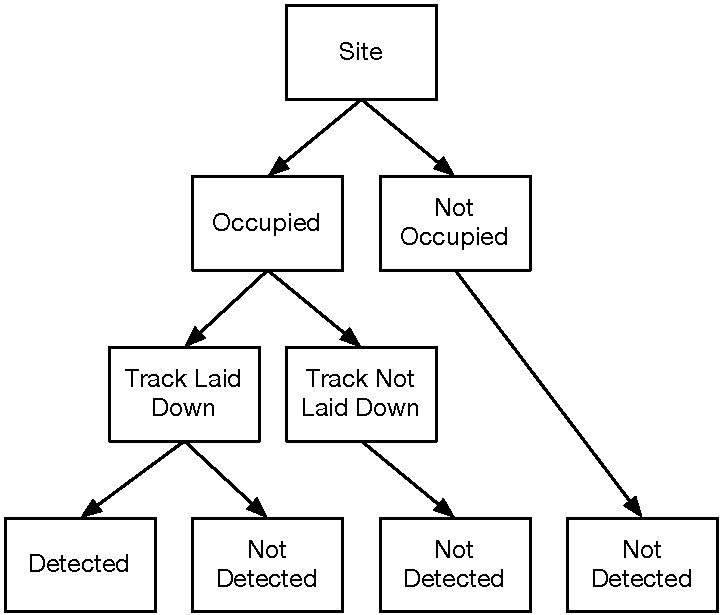
\includegraphics[scale=0.75]{Figures/Diagrams/SimpleHierarchicalModel}
        \caption{A visualization of how the hierarchical model works.}
        \label{simplehierarchicalmodel}
    \end{center}
    \end{figure}

    Figure \ref{simplehierarchicalmodel} suggests that we need separate
    parameters for (i) the probability that a plot is occupied, (ii) the
    probability that a track is laid
    down given that a plot is occupied, and (iii) the probability of detection
    given that a track is laid down and the plot is occupied. We notate
    these as \(\psi\), \(\theta\), and \(p\), respectively.

\section{Exploring the data}

    \subsection{Descriptive statistics}
    In 2003, three different observers flew over the rivers. Assuming that no
    tracks are laid down between individuals' flights on the same day, all three
    people should have seen the same tracks. While there is some error in
    classifying in which plot the observer saw the actual track, each observer
    should at least be seeing the same, or nearly the same, number of plots with
    tracks. However, we did not find that to be the case. If we look only at
    days that all three people observed, there appear to be major differences
    among the proportion of plots in which the observers detected a track
    (Figure \ref{obsPlots}). The difference in estimated na\"ive occupancy among
    the
    observers indicates that the observers did not always correctly identify
    the tracks.

    \begin{figure}
        \centering
        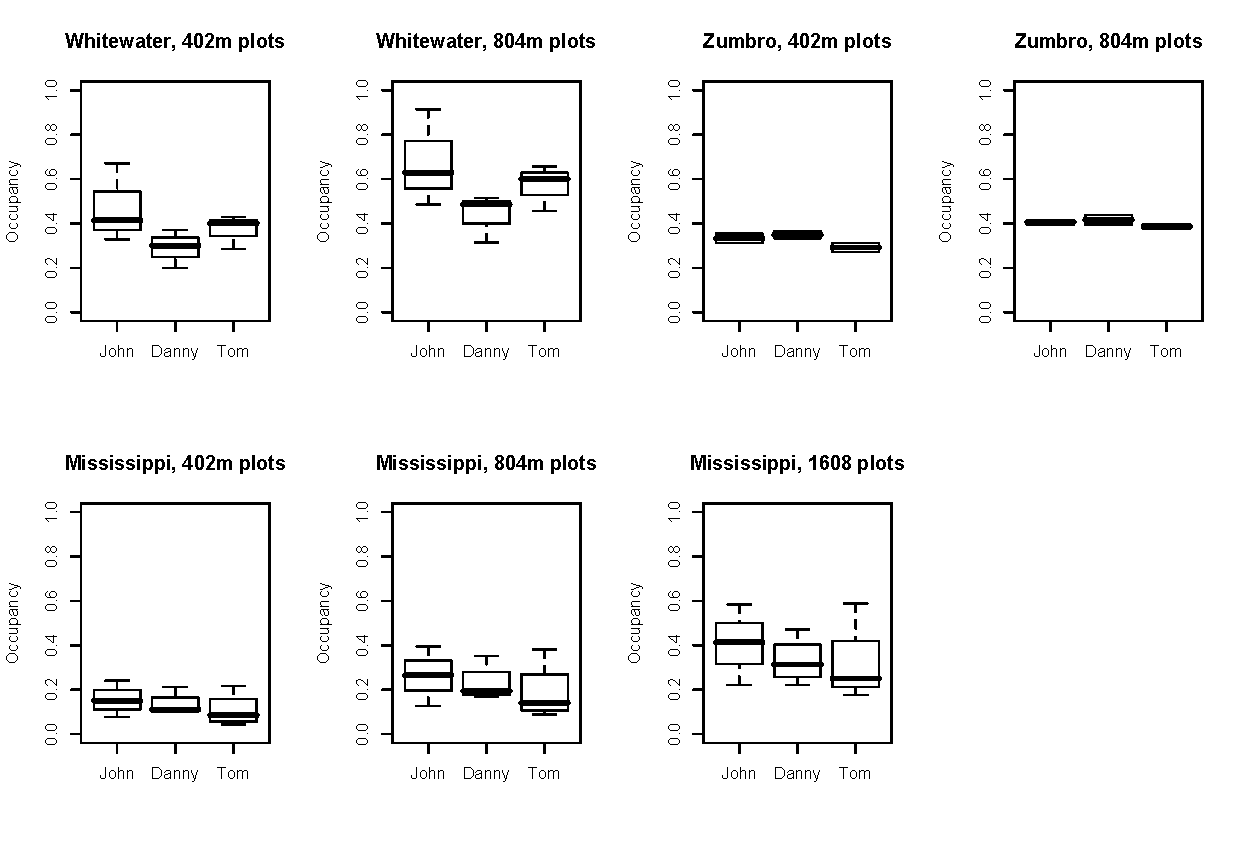
\includegraphics[width=5in]{Figures/R/observerPlots.pdf}
        \caption{The box plots show how the proportion of plots in which an
        observer saw tracks (``occupancy'') differs among the three observers in
        2003. Only those dates on which all three observers flew are included.}
        \label{obsPlots}
    \end{figure}

    Correlation among the flight sequences is low. For example, average
    correlation between flights on the Mississippi in 2003 is 0.176 for 402
    meter plots. Some of this is due to the difficulties in determining to which
    plot each track belongs. However, we have also found quite a bit of
    variation in the data not necessarily due to these classification issues.
    This is difficult to quantify. Correlation between flights is a bit higher
    for
    flights on the same day or flights during the same snow event, but still not
    as high as one might expect. Correlation rarely exceeds 0.5. The proportion
    of plots with tracks detected
    generally increases with days since snow, likely because the otters have a
    longer time to lay down a track as time after the snow event passes.

    \subsection{False positive rates}
    The lack of consistency among the flights is strong evidence that the data
    contain false positives where observers think they see a track when it does
    not exist. Not accounting for such a process can lead to major biases; as
    the number of flights increases, the occupancy rate estimate will approach
    1 \cite{Royle2006}. We thus introduced a false detection process whereby an 
    observer
    can mark down the existence of a track when in reality there is none. This
    false detection process can occur as long as there is no track, whether or
    not the plot is occupied.

    \subsection{Testing the independence assumption}
    \label{shat}
    Since one of the assumptions of occupancy modeling is that there is
    independence between plots, we wanted to see if this assumption held true
    for our data.  In order to do this, we proposed the statistic \(S\), which
    we define as the number of successive \(0\)--\(1\)'s minus the number of
    successive \(1\)--\(1\)'s per flight. Under the null hypothesis that each
    plot is an independent Bernoulli trial where \(p\) is the probability of a
    \(1\) we were able
    to compute the mean and standard deviation of \(S\), which we used to
    calculate a Z-score, where \(Z = (S - E[S])/SD[S]\). In order to
    compute these values, we needed to find the
    expected value and variance of \(S\). These calculations can be
    found in Appendix \ref{math}.

    Simulations show that the distribution of \(S\) is roughly normal.
    Using our calculations for the mean and the standard deviation, we
    computed a Z-score for each flight, where we use a plug-in estimate for
    \(p\) to be the proportion of \(1\)'s per flight. \(|Z| > 2\) suggests that
    the assumption of
    independence between plots is violated for that flight, and we found that a
    large number of flights show a significant departure from independence. We
    found that, in
    general, data with alternating plots are more ``independent'' than all plots
    as measured
    by this statistic. However, alternating plots do not guarantee independence.
    For instance, six of eleven flights along the Zumbro River during 2003 still
    have significant Z-scores with alternating plots (Table \ref{Z-scores}). It
    also appears that there
    may be slightly more independence when larger plot sizes are used, although
    it is not clear if this trend is significant. There
    were no noticeable trends for this statistic with respect to observer, days
    since snow, or snow event.

    % Mississippi River!
    \begin{table}
    \caption{Summary of \(\hat{S}\) Z-scores}
    \label{Z-scores}
    \begin{center}
    \begin{tabular}{|l|l|l|l|l|}
        \hline
        \multicolumn{5}{|l|}{\textbf{Mississippi River}} \\
        \hline
        \multirow{2}{*}{Year} & \multirow{2}{*}{Size} & \multirow{2}{*}{Flights}
        & \multicolumn{2}{|l|}{\# Sig. Z-Scores} \\
        \cline{4-5}
        & & & All Plots & Alt. Plots \\
        \hline
        \multirow{3}{*}{2003} & 402m & \multirow{3}{*}{20} & 7 & 0 \\
        \cline{2-2} \cline{4-5}
        & 804m & & 5 & 0 \\
        \cline{2-2} \cline{4-5}
        & 1608m & & 1 & 0 \\
        \hline
        \multirow{3}{*}{2004} & 402m & \multirow{3}{*}{6} & 5 & 3 \\
        \cline{2-2} \cline{4-5}
        & 804m & & 3 & 0 \\
        \cline{2-2} \cline{4-5}
        & 1608m & & 2 & 0 \\
        \hline
    \end{tabular}
    \end{center}

    % Whitewater River!
    \begin{center}
    \begin{tabular}{|l|l|l|l|l|}
        \hline
        \multicolumn{5}{|l|}{\textbf{Whitewater River}} \\
        \hline
        \multirow{2}{*}{Year} & \multirow{2}{*}{Size} & \multirow{2}{*}{Flights}
        & \multicolumn{2}{|l|}{\# Sig. Z-Scores} \\
        \cline{4-5}
        & & & All Plots & Alt. Plots \\
        \hline
        \multirow{2}{*}{2003} & 402m & \multirow{2}{*}{15} & 6 & 2 \\
        \cline{2-2} \cline{4-5}
        & 804m & & 4 & 1 \\
        \hline
        \multirow{2}{*}{2004} & 402m & \multirow{2}{*}{6} & 3 & 1 \\
        \cline{2-2} \cline{4-5}
        & 804m & & 2 & 2 \\
        \hline
    \end{tabular}
    \end{center}

    % Zumbro River!
    \begin{center}
    \begin{tabular}{|l|l|l|l|l|}
        \hline
        \multicolumn{5}{|l|}{\textbf{Zumbro River}} \\
        \hline
        \multirow{2}{*}{Year} & \multirow{2}{*}{Size} & \multirow{2}{*}{Flights}
        & \multicolumn{2}{|l|}{\# Sig. Z-Scores} \\
        \cline{4-5}
        & & & All Plots & Alt. Plots \\
        \hline
        \multirow{2}{*}{2003} & 402m & \multirow{2}{*}{11} & 10 & 6 \\
        \cline{2-2} \cline{4-5}
        & 804m & & 8 & 5 \\
        \hline
        \multirow{2}{*}{2004} & 402m & \multirow{2}{*}{4} & 3 & 3 \\
        \cline{2-2} \cline{4-5}
        & 804m & & 3 & 1 \\
        \hline
    \end{tabular}
    \end{center}
    \end{table}

    We think that the lack of independence results from strings of ones where an
    otter left a track across multiple plots. When alternating plots are used,
    the strings are cut in half and the occurrence of \(1\)--\(1\)'s is lower
    while the occurrence of \(0\)--\(1\)'s stays about the same. It is
    noteworthy that virtually all the violations of independence are in the
    direction of more \(1\)--\(1\)'s than would be expected. We believe that
    successive \(1\)'s could represent a single track made by the same otter. We
    will
    discuss later how sensitive our model is to this violation of independence,
    and how this might affect the estimation of actual occupancy rates.

\section{Bayesian modeling theory and practice}

    \subsection{Bayesian statistics}
    Most occupancy models utilize maximum likelihood estimation, but we chose
    to use a Bayesian approach to model the data for several reasons.
    First, the occupancy models developed using maximum likelihood methods
    assume that the sampled locations are a random sample from a large,
    theoretically infinite, population.  In this study, the entire area of
    interest was observed, so this assumption does not hold true.  Bayesian
    models do not make such an assumption.  Second, because our model added
    extra
    parameters, formulating the likelihood function was cumbersome and
    maximizing
    it would have been difficult.  We added an additional random process, track
    laying, and also included the possibility of false detection.  A Bayesian
    model seems much more intuitive and natural.

    Once we had a model formulated, we could then use Markov Chain Monte Carlo
    (MCMC) to find a posterior distribution for every parameter. Due to the
    nature of occupancy models, certain models can have multiple
    interpretations.
    We run into one such duality with the probability of correct detection
    \(p\), and the probability of false detection \(E\). These two variables
    have bimodal posterior distributions, because \((p=x,E=y,\psi=z)\) is
    equivalent in terms of likelihood to \((p=y,E=x,\psi=1-z)\) due to the
    symmetry of the model \cite{Royle2006}.  Since it is reasonable
    for \(p\) to be greater than \(E\), we solved this problem by restricting
    the distribution of \(p\) to the range \((0.6,1)\), and \(E\) to
    \((0,0.4)\), an adaptation of the approach recommended by Royle and
    Link \cite{Royle2006}.

    \subsection{WinBUGS/R}
    To implement a Bayesian hierarchical model, we make use of the software
    packages WinBUGS \cite{Lunn2000}, R \cite{R2009}, BRugs \cite{Thomas2008},
    and, by extension, OpenBUGS \cite{Thomas2006}. One can describe the model
    using an ``intuitive `pseudo-code' representation'' in WinBUGS
    \cite{MacKenzie2006} and then run the model within the familiar environment
    of R using the combination of BRugs and OpenBUGS. OpenBUGS, the open source,
    cross-platform successor to WinBUGS, uses the same syntax. All of the
    aforementioned software packages are open source and available
    freely\footnote{WinBUGS: \url{http://www.mrc-bsu.cam.ac.uk/bugs/} and R:
    \url{http://www.r-project.org/} are available as standalone programs. The
    BRugs/OpenBUGS package can be installed by typing
    \texttt{install.packages("BRugs")} in R's interactive shell. Note that while
    R and OpenBUGS include official support for Mac OS X and Unix/Unix-like
    operating systems, WinBUGS and the BRugs package are only available for
    Windows.}.

    WinBUGS requires a representation of a model, data, and initial values on
    which a predetermined number of iterations of the MCMC algorithm are
    executed \cite{MacKenzie2006}.
    The data we received from the
    Minnesota Department of Natural Resources was unbalanced with regard to
    covariates.
    Our initial simulations, on the other
    hand, ran on data sets with a fixed number of observers, snow events, and
    observations after each snow event, which are much easier to implement
    within WinBUGS and R.

\section{Standard hierarchical model}

    \subsection{Our hierarchical model}
    For our model, we specified noninformative uniform \((0, 1)\) prior
    distributions for
    parameters \(\psi\) and \(\theta\), a common, natural choice given a lack of
    formal information about the prior or expert consensus \cite{MacKenzie2006}.
    We implemented models with normal and beta prior distributions on \(p\) and
    \(E\) and limited the range of \(p\) to the interval \((0.6, 1)\) and the
    range of \(E\) to the interval \((0, 0.4)\) in both models. We set the
    burn-in time for the MCMC simulation to 10,000 iterations, which seemed
    necessary to handle convergence. Each of these
    parameters are tracked for 10,000 additional iterations and are estimated
    by the mean of the posterior distribution. The covariates of this
    model are the observer and the number of days since the last snow event.
    It was necessary to preprocess the Minnesota DNR's data to account for its
    irregularities.

    \subsection{Simulated data}
    We simulated both balanced and unbalanced data sets meant for the standard
    hierarchical model with given values of \(\psi\), \(\theta\), \(p\) for each
    observer, and \(E\) for each observer.  Balanced data sets, in this context,
    contain the same number of flights by the same observers after each snow
    event.

    To simulate balanced data, we provided the following additional variables:
    the number of plots, the number of snow events, the number of observers, and
    the number of observations following each snow event. These variables are
    all that are required to allow us to generate data in which each snow event
    receives the same number of flights by the same number of observers, which
    greatly simplifies the accompanying hierarchical model. For the simulation,
    we first determine each plot's occupancy status based
    based upon the given \(\psi\) value.
    Then, for each day after each snow event, the simulation decides whether or
    not an otter laid down a track. For a given day after a snow event, a track
    is considered to be present if an otter lays a track down on any of the days
    after the snow event up to and including the given day. Once that has been
    decided, the given \(p\) and \(E\) values are used to assign a 0 (not
    detected) or 1 (detected).

    Because of limitations with respect to WinBUGS' syntax, simulating
    unbalanced data requires additional information and a reformatting
    of the data as well as the corresponding hierarchical model. While the
    resulting code's structure differs from that used for balanced
    data, the underlying model remains the same.

    To determine the efficacy of the standard model over the range of possible
    \(\psi\) and \(\theta\) values, we ran simulations with several combinations
    of \(\psi\) and \(\theta\), ran the model on each simulation, and compared
    the model's estimates to the simulation's parameters (Table \ref{Simulated
    data}). The model with beta
    prior distributions on \(p\) and \(E\) performed better than the model with
    normal prior distributions on the same parameters. The beta distribution
    gives a flexible two-parameter family of distributions on \((0,1)\). We
    included two hyper-parameters (\(\alpha\) and \(\beta\)) on the beta
    distribution as part of our hierarchical modeling, which seemed to work
    well.

    \begin{table}
    \caption{Model estimates from simulated data. All simulations
    ran with 70 plots, 5 snow events, 3 observers, and for 3 days after each
    snow event. The 3 observers had \(p\) values of 0.70, 0.80, 0.90 and \(E\)
    values of 0.05, 0.20, and 0.30, respectively. Green rows represent values of
    \(\psi\) and \(\theta\) for which the model exhibits good convergence and
    the 95\% confidence interval captures the actual \(\psi\) value.  Yellow
    rows represent values for which our model exhibits either mediocre
    convergence or a bad confidence interval.  Red rows represent values for
    which our model does not converge.}
    \label{Simulated data}
    \begin{center}
    \begin{tabular}{|l|l|l|l|}
        \hline
            \(\psi\) & \(\theta\) & Convergence & 95\% CI (\(\psi\)) \\
        \hline
        \multirow{5}{*}{0.20}
            & \cellcolor{Green}0.20 & \cellcolor{Green}Good &
              \cellcolor{Green}(0.112, 0.305) \\
            & \cellcolor{Green}0.40 & \cellcolor{Green}Good &
              \cellcolor{Green}(0.142, 0.341) \\
            & \cellcolor{Green}0.60 & \cellcolor{Green}Good &
              \cellcolor{Green}(0.098, 0.284) \\
            & \cellcolor{Green}0.80 & \cellcolor{Green}Good &
              \cellcolor{Green}(0.097, 0.281) \\
            & \cellcolor{Yellow}1.00 & \cellcolor{Yellow}Okay &
              \cellcolor{Yellow}(0.117, 0.302) \\
        \hline
        \multirow{5}{*}{0.40}
            & \cellcolor{Yellow}0.20 & \cellcolor{Yellow}Okay &
              \cellcolor{Yellow}(0.388, 0.721) \\
            & \cellcolor{Green}0.40 & \cellcolor{Green}Good &
              \cellcolor{Green}(0.270, 0.494) \\
            & \cellcolor{Green}0.60 & \cellcolor{Green}Good &
              \cellcolor{Green}(0.287, 0.512) \\
            & \cellcolor{Red}0.80 & \cellcolor{Red}Bad &
              \cellcolor{Red}(0.277, 0.507) \\
            & \cellcolor{Yellow}1.00 & \cellcolor{Yellow}Okay &
              \cellcolor{Yellow}(0.279, 0.503) \\
        \hline
        \multirow{5}{*}{0.60}
            & \cellcolor{Yellow}0.20 & \cellcolor{Yellow}Good &
              \cellcolor{Yellow}(0.312, 0.581) \\
            & \cellcolor{Green}0.40 & \cellcolor{Green}Good &
              \cellcolor{Green}(0.400, 0.630) \\
            & \cellcolor{Yellow}0.60 & \cellcolor{Yellow}Okay &
              \cellcolor{Yellow}(0.462, 0.687) \\
            & \cellcolor{Yellow}0.80 & \cellcolor{Yellow}Okay &
              \cellcolor{Yellow}(0.502, 0.727) \\
            & \cellcolor{Red}1.00 & \cellcolor{Red}Bad &
              \cellcolor{Red}(0.318, 0.549) \\
        \hline
        \multirow{5}{*}{0.80}
            & \cellcolor{Green}0.20 & \cellcolor{Green}Good &
              \cellcolor{Green}(0.578, 0.838) \\
            & \cellcolor{Green}0.40 & \cellcolor{Green}Good &
              \cellcolor{Green}(0.736, 0.915) \\
            & \cellcolor{Yellow}0.60 & \cellcolor{Yellow}Okay &
              \cellcolor{Yellow}(0.587, 0.829) \\
            & \cellcolor{Yellow}0.80 & \cellcolor{Yellow}Okay &
              \cellcolor{Yellow}(0.599, 0.811) \\
            & \cellcolor{Red}1.00 & \cellcolor{Red}Bad &
              \cellcolor{Red}(0.612, 0.830) \\
        \hline
        \multirow{5}{*}{1.00}
            & \cellcolor{Yellow}0.20 & \cellcolor{Yellow}Good &
              \cellcolor{Yellow}(0.895, 0.999) \\
            & \cellcolor{Yellow}0.40 & \cellcolor{Yellow}Okay &
              \cellcolor{Yellow}(0.927, 0.999) \\
            & \cellcolor{Green}0.60 & \cellcolor{Green}Good &
              \cellcolor{Green}(0.949, 1.000) \\
            & \cellcolor{Yellow}0.80 & \cellcolor{Yellow}Good &
              \cellcolor{Yellow}(0.802, 0.954) \\
            & \cellcolor{Red}1.00 & \cellcolor{Red}Bad &
              \cellcolor{Red}(0.800, 0.955) \\
        \hline
    \end{tabular}
    \end{center}
    \end{table}

    Generally, the model is most effective for lower values of \(\psi\) and
    \(\theta\) but will either converge well or provide useful estimates for the
    vast majority of combinations of \(\psi\) and \(\theta\) values. Twenty-one
    of the
    model's 25 confidence intervals for \(\psi\) capture the actual value.
    The model's confidence intervals for each of the
    three values of \(p\) include its actual value for all \(\psi\) and
    \(\theta\) values. On the other hand, the model accurately estimates \(E\)
    for low values of \(\theta\), but consistently overestimates \(E\) when
    \(\psi\geq0.4\) and \(\theta\geq0.6\) regardless of \(E\)'s actual value.
    This may help to explain why the model does not estimate \(\psi\) as
    successfully for higher values of \(\psi\) and \(\theta\).

\section{Spatial correlation of the data}
One approach to dealing with the correlation in the
observed tracks in neighboring plots is to use a conditional autoregressive
(CAR) prior distribution for $\theta$, the probability that an otter lays down a
track in a plot on a given day.

    \subsection{Conditional autoregressive (CAR) models}
    Let $\theta_s$ be the probability of a track being laid down in plot $s$ on
    a given day. Then the Gaussian CAR model can be defined using the following
    conditional distributions:
    \begin{equation}
        \theta_s|\theta_i,\tau_s^2 \sim N(\mu_s+\sum_{i\in N_s}
        c_{si}(y_i-\mu_i),\tau_s^2)
    \end{equation}
    where $N_s$ is the set of neighbors of area $s$ (in this case, the two
    bordering plots), $E(\theta_s)=\mu_s$, $\tau_s^2$ is the conditional
    variance, $c_{si}$ is the weight defining how strong the correlation is
    between plots $s$ and $i$, and $c_{ii}=0$ for all plots $i$ \cite{Arab2008}.
    Essentially, this model means that if plot $s$'s neighbor has a
    particularly high or low track-laying probability, that will increase or
    decrease the track-laying probability for plot $s$. This makes it more
    likely to have strings of tracks that cross over multiple plots.

    \subsection{Our CAR model}
    \label{car model}
    For our model, both neighbors are weighted equally. Since $\tau_s$ for any
    plot $s$ is unknown, we followed convention and used the same value of
    $\tau$ for all plots and placed a prior distribution on it. We chose a
    $\gamma(0.5,0.0005)$ prior distribution for $(\tau^2)^{-1}$, a common choice
    \cite{Thomas2004}. In our model we define $\text{logit}(\theta_s)=\alpha_0+
    \alpha_{1_s}$ where $\alpha_0$ has an improper uniform distribution and
    $\alpha_1$ has a Gaussian CAR distribution. We again used a uniform prior
    distribution on $\psi$ and the same beta prior distributions on $p$ and $E$.
    In this case, we limited the range of $p$ to the interval $(0.6,1)$ and the
    range of $E$ to $(0,0.3)$. We increased the burn-in time to 12,000
    iterations. With this model, instead of a single estimate for $\theta$ there
    are now $n$ estimates for $\theta$ where $n$ is the total number of plots.
    While ideally we would estimate an overall value for $\theta$, it seems more
    important for the purposes of this investigation to estimate $\psi$.

    \subsection{Simulating spatially correlated data}
    \label{spatial simulation}
    We began by simulating
    spatial correlation in the track-laying process. To do this, we added an
    additional variable, $\alpha$, to the simulated data. Under the new
    simulation method, $\theta$ is the probability of an otter laying down a
    track in plot $i$ given plot $i$ is occupied and plot $i-1$ does
    \textit{not} have a track. If plot $i$ is occupied and plot $i-1$ does have
    a track, then the probability of an otter laying down a track in plot $i$ is
    equal to $\theta+\alpha$. This means if there is a track in one plot, there
    is more likely to be a track in the next plot. However, when we ran data
    simulated using this new method on the model described in Section \ref{car
    model}, the model almost never converged. We tested independence of the data
    using the $S$ statistic we developed (Section \ref{shat}) and found
    that the simulated data displayed much less dependence than the actual
    data. We would like our simulated data to have the same level of dependence
    as our actual data.  We tried modeling spatial correlation in the occupancy
    process, $\psi$, instead of in the track-laying process, but the simulated
    data were again more independent than the real data.

    To increase the correlation between plots we simulated the correlation
    in both the track-laying and occupancy processes. Under this 
    simulation method we
    again had the variables $\theta$ and $\alpha$, but we also had analogous
    variables $ \psi$ and $\beta$. In this case, $\psi$ is the probability an
    otter occupies plot $i$ given that plot $i-1$ is not occupied and $\psi+
    \beta$ is the probability that an otter occupies plot $i$ given that plot
    $i-1$ is occupied. With this increased spatial correlation we were able to
    more closely match the $S$-related Z-scores found in the actual data. In
    addition, the CAR model converged more often with data simulated using this
    method, but it still did not converge consistently. When it did converge,
    estimates were comparable to those found using the standard model on the
    same simulated data.

    When we ran the data with spatial correlation in the occupancy process on
    the CAR model, we could no longer compare the model estimate for $\psi$ to
    the simulated value of $\psi$ because they had different meanings. To get a
    sense of the overall occupancy rate in the simulated data we counted the
    number of plots that were occupied (known because the data are simulated)
    and divided that by the total number of plots. This proportion is the value
    we compared to the $\psi$ estimate from both hierarchical models.

\section{Discussion}

    \subsection{Obtaining convergence on the data}
    Once both the standard hierarchical model and the addition of a CAR prior
    distribution on \(\theta\) to the standard model exhibited convergence on
    our simulated data, we moved on to running both models on the actual data.
    In general, the sparseness of the data gathered in 2004 caused us to
    simplify the model in order to obtain results. Unfortunately, the
    simplification results in estimates of \(\psi\) that do not seem accurate
    and are not directly comparable to estimates of \(\psi\) on 2003's data.

    The standard model converged reliably on all data gathered in 2003, but it
    did not converge on any of the data gathered in 2004. Considering that the
    amount of data gathered in 2004 pales in comparison to the amount of data
    gathered in 2003, this result was not surprising. The vast majority of
    2004 data consists of just one observer taking observations once after
    each snow event, which causes \(p\) and \(E\) in particular to not converge,
    regardless of plot size.

    To obtain convergence on 2004 data, we removed \(E\), thus disallowing false
    positives. Although the model still did not
    converge on data with plot sizes of 804m and 1608m, both the Whitewater and
    Zumbro Rivers' data at the 402m plot size converged. Although none of the
    Mississippi River's 2004 data converged, we still include estimates of
    \(p\), \(\psi\), and \(\theta\) at the 402m plot size to accompany the
    estimates corresponding to the Whitewater and Zumbro Rivers. For the most
    part, however, we feel that the absence of \(E\) from the model makes the
    the estimates of \(\psi\) less dependable.

    The addition of a CAR prior distribution on \(\theta\) to the standard model
    caused the model to fail to converge on all of the data. Although the
    standard model and the CAR model performed similarly on simulated data
    whenever both models converged, the standard model converged much more often
    than did the CAR model. This is most likely due to the fact that the CAR
    model attempts to estimate many more parameters. Whereas the standard model
    estimates between eight and twelve parameters on the actual data (\(\psi\),
    \(\theta\), the four parameters of the beta distributions corresponding to
    \(p\) and \(E\), \(p\) for each observer, and \(E\) for each observer), the
    CAR model estimates \(\theta\) for each plot. Because there are at least
    thirty-five plots in each data set (regardless of plot size), the CAR prior
    distribution adds a considerable amount of complexity to the model.

    We also tried to simplify this model by eliminating \(E\) because this was
    somewhat successful with respect to convergence with the standard model. We
    first attempted to fit this model to data from 2003 at the 402m plot size.
    Although the model successfully converged on all of this data, its estimates
    of \(\psi\), all of which were greater than 0.9, did not seem reasonable,
    especially in comparison to the standard model's estimates when given the
    same data. As a result, we did not attempt to fit this model to the rest of
    the data and do not include this model's estimates within our results.

    % Mississippi River!
    \begin{table}
    \caption{Mississippi River. 2003 data converged well at the 402m and 804m
    plot sizes. At the 1608m plot size, \(E\), \(\psi\), and \(\theta\) did not
    converge well. 2004 data did not converge. We do not think that these
    estimates are accurate, but they are included for the sake of completeness.}
    \label{Mississippi}
    \begin{center}
    \begin{tabular}{|l|l|l|l|}
        \hline
        \multicolumn{4}{|l|}{\textbf{Mississippi River, 2003}} \\
        \hline
            & 402m & 804m & 1608m \\
        \hline
        \multirow{2}{*}{E[Danny]}
            & 0.01954 & 0.04808 & 0.06885 \\
            & (0.006515, 0.03663) & (0.01874, 0.08187) & (0.01778, 0.1383) \\
        \hline
        \multirow{2}{*}{E[John]}
            & 0.05216 & 0.07771 & 0.13650 \\
            & (0.027710, 0.07745) & (0.03881, 0.12100) & (0.03449, 0.2330) \\
        \hline
        \multirow{2}{*}{E[Tom]}
            & 0.02668 & 0.06140 & 0.10230 \\
            & (0.011990, 0.04622) & (0.02789, 0.10390) & (0.04287, 0.1796) \\
        \hline
        \multirow{2}{*}{p[Danny]}
            & 0.65240 & 0.67340 & 0.74960 \\
            & (0.548300, 0.75990) & (0.56760, 0.78290) & (0.60510, 0.8910) \\
        \hline
        \multirow{2}{*}{p[John]}
            & 0.67770 & 0.77580 & 0.82540 \\
            & (0.583500, 0.77280) & (0.66060, 0.88690) & (0.71390, 0.9326) \\
        \hline
        \multirow{2}{*}{p[Tom]}
            & 0.53670 & 0.54220 & 0.65330 \\
            & (0.501200, 0.61300) & (0.50160, 0.62850) & (0.51530, 0.8104) \\
        \hline
        \multirow{2}{*}{\(\psi\)}
            & 0.59380 & 0.69370 & 0.75820 \\
            & (0.439000, 0.75990) & (0.51800, 0.87380) & (0.54110, 0.9300) \\
        \hline
        \multirow{2}{*}{\(\theta\)}
            & 0.15280 & 0.20730 & 0.27690 \\
            & (0.111900, 0.19780) & (0.14580, 0.27390) & (0.19030, 0.3716) \\
        \hline
    \end{tabular}
    \end{center}

    \begin{center}
    \begin{tabular}{|l|l|}
        \hline
        \multicolumn{2}{|l|}{\textbf{Mississippi River, 2004}} \\
        \hline
            & 402m \\
        \hline
        \multirow{2}{*}{p[Danny]}
            & 0.3129 \\
            & (0.2174, 0.8107) \\
        \hline
        \multirow{2}{*}{\(\psi\)}
            & 0.7613 \\
            & (0.6609, 0.8833) \\
        \hline
        \multirow{2}{*}{\(\theta\)}
            & 0.8511 \\
            & (0.2426, 0.9973) \\
        \hline
    \end{tabular}
    \end{center}
    \end{table}

    % Whitewater River!
    \begin{table}
    \caption{Whitewater River. In 2003, while the 402m data converged well,
    \(E\), \(\psi\), and \(\theta\) did not converge well for the 804m data.
    2004 data converged well. However, we feel that the absence of \(E\) from
    the model makes the estimates much less dependable. The estimates are also
    much less precise than those from 2003 -- the confidence intervals of
    \(\psi\) and of \(p[Danny]\) are twice as large as those from 2003.}
    \label{Whitewater}
    \begin{center}
    \begin{tabular}{|l|l|l|}
        \hline
        \multicolumn{3}{|l|}{\textbf{Whitewater River, 2003}} \\
        \hline
            & 402m & 804m \\
        \hline
        \multirow{2}{*}{E[Danny]}
            & 0.05608 & 0.0555 \\
            & (0.02474, 0.09554) & (0.002859, 0.1390) \\
        \hline
        \multirow{2}{*}{E[John]}
            & 0.16570 & 0.1931 \\
            & (0.10130, 0.23510) & (0.065910, 0.3384) \\
        \hline
        \multirow{2}{*}{E[Tom]}
            & 0.15350 & 0.2241 \\
            & (0.09758, 0.21660) & (0.110000, 0.3623) \\
        \hline
        \multirow{2}{*}{p[Danny]}
            & 0.66990 & 0.6985 \\
            & (0.56080, 0.79040) & (0.573100, 0.8366) \\
        \hline
        \multirow{2}{*}{p[John]}
            & 0.92040 & 0.9877 \\
            & (0.84270, 0.97590) & (0.945100, 1.0000) \\
        \hline
        \multirow{2}{*}{p[Tom]}
            & 0.75910 & 0.8575 \\
            & (0.65060, 0.85800) & (0.745400, 0.9600) \\
        \hline
        \multirow{2}{*}{\(\psi\)}
            & 0.87590 & 0.9126 \\
            & (0.72910, 0.98880) & (0.746900, 0.9955) \\
        \hline
        \multirow{2}{*}{\(\theta\)}
            & 0.24100 & 0.3779 \\
            & (0.17890, 0.30900) & (0.286500, 0.4721) \\
        \hline
    \end{tabular}
    \end{center}

    \begin{center}
    \begin{tabular}{|l|l|l|l|}
        \hline
        \multicolumn{2}{|l|}{\textbf{Whitewater River, 2004}} \\
        \hline
            & 402m \\
        \hline
        \multirow{2}{*}{p[Danny]}
            & 0.8237 \\
            & (0.5323, 0.9804) \\
        \hline
        \multirow{2}{*}{\(\psi\)}
            & 0.6066 \\
            & (0.4246, 0.8382) \\
        \hline
        \multirow{2}{*}{\(\theta\)}
            & 0.2068 \\
            & (0.1211, 0.3550) \\
        \hline
    \end{tabular}
    \end{center}
    \end{table}

    % Zumbro River!
    \begin{table}
    \caption{Zumbro River. In 2003, the 402m data converged well. While \(\psi\)
    and \(\theta\) converged well for the 804m data, none of the other
    parameters did. 2004 data converged well. However, as is the case with all
    of the 2004 data, we feel that the absence of \(E\) from the model makes the
    estimates much less dependable.}
    \label{Zumbro}
    \begin{center}
    \begin{tabular}{|l|l|l|}
        \hline
        \multicolumn{3}{|l|}{\textbf{Zumbro River, 2003}} \\
        \hline
            & 402m & 804m \\
        \hline
        \multirow{2}{*}{E[Danny]}
            & 0.02922 & 0.007066 \\
            & (0.006786, 0.05994) & (0.0000, 0.03403) \\
        \hline
        \multirow{2}{*}{E[John]}
            & 0.03388 & 0.008312 \\
            & (0.008584, 0.06880) & (0.0000, 0.04188) \\
        \hline
        \multirow{2}{*}{E[Tom]}
            & 0.02228 & 0.012960 \\
            & (0.002430, 0.05385) & (0.0000, 0.05642) \\
        \hline
        \multirow{2}{*}{p[Danny]}
            & 0.81890 & 0.837100 \\
            & (0.749500, 0.88540) & (0.7615, 0.90700) \\
        \hline
        \multirow{2}{*}{p[John]}
            & 0.81770 & 0.852500 \\
            & (0.740100, 0.88670) & (0.7597, 0.92230) \\
        \hline
        \multirow{2}{*}{p[Tom]}
            & 0.73120 & 0.805400 \\
            & (0.625400, 0.82440) & (0.6885, 0.89780) \\
        \hline
        \multirow{2}{*}{\(\psi\)}
            & 0.66550 & 0.651600 \\
            & (0.549100, 0.78150) & (0.5098, 0.78210) \\
        \hline
        \multirow{2}{*}{\(\theta\)}
            & 0.29950 & 0.395800 \\
            & (0.236400, 0.36550) & (0.3100, 0.48520) \\
        \hline
    \end{tabular}
    \end{center}

    \begin{center}
    \begin{tabular}{|l|l|l|l|}
        \hline
        \multicolumn{2}{|l|}{\textbf{Zumbro River, 2004}} \\
        \hline
            & 402m \\
        \hline
        \multirow{2}{*}{p[Danny]}
            & 0.9166 \\
            & (0.7739, 0.9918) \\
        \hline
        \multirow{2}{*}{\(\psi\)}
            & 0.4773 \\
            & (0.3586, 0.6114) \\
        \hline
        \multirow{2}{*}{\(\theta\)}
            & 0.4232 \\
            & (0.3073, 0.5520) \\
        \hline
    \end{tabular}
    \end{center}
    \end{table}

    \subsection{Summary and interpretation of estimates}
    Tables \ref{Mississippi}, \ref{Whitewater}, and \ref{Zumbro} contain our
    estimates for all of the data from
    2003 and 2004.
    With respect to the model's ability to converge on the actual data, the most
    important factors are plot size, the number of flights recorded, and the
    number of estimated parameters. In general, both plot size and the number of
    flights recorded must be sufficiently small and large, respectively, for the
    standard model with \(E\) to converge.

    The 2003 data worked relatively well with the model. The presence of
    numerous
    observations that occur in the second and third days since the most recent
    snow event allows one of the more crucial assumptions of our hierarchical
    model -- that otter tracks laid on each day after a snow event are visible
    throughout the entire observation period and therefore, that it is more
    likely for an observer to detect a track on later days -- to be thoroughly
    tested. Most of the \(\psi\) and \(\theta\) estimates of 2003's data fall
    into ranges where our model is at its best, both with respect to convergence
    and to accurately estimating \(\psi\).

    The 2004 data, which suffered from the lack of multiple observers and
    observations later than one day after each snow event, does not provide
    enough data with respect to time (measured by the number of days since the
    last snow event) for the parameters \(p\) and \(E\) to converge, regardless
    of the number of MCMC iterations performed.

    As plot size increases, every estimated parameter tends to increase as well.
    Although the vast majority of these increases, even at the 1608m plot size,
    lie well within the 95\% confidence interval of the accompanying estimate at
    the 402m plot size, we believe that this trend makes sense. Only one track
    detection within a plot is necessary to assign it a 1. Therefore, once 402m
    plots are aggregated into 1608m plots, only one of the four 402m plots needs
    to be assigned a 1 in order for the entire 1608m plot to receive a 1. The
    amount of correlation between 1's determines the increase in the proportion
    of 1's to the number of plots -- as the amount of correlation increases,
    there will be more strings of 1's which are aggregated together, so the
    increase in the proportion decreases.

    We believe that this increase leads to higher \(\psi\) and \(\theta\)
    estimates because the potential for otters to lay tracks within a larger
    plot increases. There is also an increased potential for multiple otters to
    reside within a larger plot. In southeastern Minnesota, most otters tolerate
    the
    presence of other otters in the areas they use most frequently, suggesting
    that they are neither solitary nor territorial \cite{Gorman2006}. This is
    consistent with the noticeable but modest increase in \(\theta\) across plot
    sizes for all three rivers.
    However, estimates of \(\psi\) along the Whitewater and Zumbro Rivers remain
    constant, despite large increases in \(\theta\).  We have not thought of an
    explanation for this.

    Similarly, the increases in estimates of \(p\) and \(E\) seem to result from
    the general increase of tracks laid per plot as the plot size grows. As plot
    size grows and there are fewer plots, the influence of a correct or
    incorrect detection increases.  If the observer fails to see a track, he may
    observe another track in the same plot, thus correctly assigning that plot a
    1 despite failing to observe a track.  With smaller plot sizes, this case
    could result in one detected plot and one undetected plot, decreasing his
    accuracy.  A similar scenario is possible with incorrectly identified
    tracks, which would increase \(E\).

    Lastly, we decided to use the data from every plot even though we believe
    that, as a result, our data violates the assumption of independence between
    plots. However, our simulations, described in Section \ref{spatial
    simulation}, indicate that the model remains effective with spatially
    correlated data.
    Since the actual data is relatively sparse as it is, we consider the removal
    of half of it in order to preserve independence to be more harmful to the
    model than supplying the model with correlated data. Therefore, all
    estimates come
    from all of the data that we were given.

    \subsection{Recommended sampling practices}
    To determine the relative importance of the different sampling variables
    (number of observers, number of snow events, and
    number of days since the most recent snow event), we ran the standard
    hierarchical model with false detection on simulated data with values of
    \(\psi\) and
    \(\theta\) similar to the estimates of \(\psi\) and \(\theta\) from 2003
    data. We varied the numbers of observers, snow events, and observations
    after
    each snow event. We assumed that observations after each snow event will
    occur on consecutive days, starting from the first day after the snow event.
    This information helped us to find more efficient ways (with respect to
    number of flights) to gather aerial occupancy data given one, two, and three
    observers while still obtaining useful estimates from the model.

    \textbf{The number of observers appears to be the least important of the
    three
    sampling variables.} We were able to obtain accurate estimates regardless of
    the
    number of observers, as long as there were sufficient numbers of snow events
    and observations after each snow event. For one observer, at least three
    snow events and three observations on consecutive days after each snow event
    are required for the model to converge and give good estimates. For two or
    three observers, two events with three observations on consecutive days
    after each snow event is sufficient. Therefore, roughly nine, twelve, and
    eighteen flights are required to obtain good estimates for one, two, and
    three observers, respectively. Surprisingly, the most cost-effective method
    (as measured by the number of flights required) only requires one observer.

    \textbf{The number of snow events appears to be the second-most important of
    the
    three sampling variables.} Although two snow events are required, only with
    one
    observer does the addition of a third snow event noticeably affect the
    model's estimates.

    \textbf{The number of observations after each snow event appears to be the
    most
    important of the three sampling variables.} Because the model relies upon
    the
    assumption that the probability of seeing a track increases each day because
    tracks made on previous days within the same snow event can still be seen,
    this is not surprising. At least two observations after each snow event on
    consecutive days are required. Additional observations after each event help
    the model converge more quickly, but the estimates become only slightly more
    accurate.

    Additional observations after each snow event are more helpful than
    additional snow events for the first three days of observation.
    Both are much more helpful than the addition of an observer.
    Once the numbers of snow events and observations after each snow event both
    surpass three, they improve the model's estimates at roughly equal rates.
    Note, however, that increasing the number of snow events is likely to be far
    less challenging than increasing the number of observations after each snow
    event at that point.

    In summary, for future data gathering trips, we suggest using one
    observer, as long as they are relatively confident that they can correctly
    identify an otter track and distinguish an otter track from the tracks of
    other animals in the immediate area, since the model most accurately
    estimates \(p\) and \(E\) when their true values are high and low,
    respectively. With one observer, three snow events and three or four snow
    days' worth of flights per snow event would be sufficient. If the same
    observer flies twice (or more often) in one day, perhaps they could act as a
    substitute for an additional observer. This is because it is probable that,
    with one flight's worth of experience observing the given river, the
    observer's \(p\) and \(E\) would change due to their newfound familiarity
    with the river.

\section{Acknowledgments}
We would like to thank our adviser, Bob Dobrow, for all of his help and advice 
and John Fieberg and John Erb from the Minnesota Department of Natural Resources
for collecting and sharing the data as well as for offering their specific
knowledge of the subject.

\bibliographystyle{amsplain}
\bibliography{Bibliography}

\appendix
\section{Deriving the mean and standard deviation of our \(S\) statistic}
\label{math}
    Given a binary sequence \(X_1, ..., X_n\) of independently and identically
    distributed 0's and 1's, let \(A=\text{\# of successive 0-1's}\), \(B=
    \text{\# of successive 1-1's}\) and \(p=\text{the proportion of 1's in the
    sequence}\). In order to find \(E[S]\), we first needed to find \(E[A]\) and
    \(E[B]\).

    % E[A]
    \begin{equation*}
        \begin{split}
        E[A]& =\sum_{i=1}^{n-1}P(X_i=0,X_{i+1}=1) \\
            & =\sum_{i=1}^{n-1}(1-p)p \\
            & =(n-1)(1-p)p \\
        \end{split}
    \end{equation*}

    % E[B]
    \begin{equation*}
        \begin{split}
        E[B]& =\sum_{i=1}^{n-1}P(X_i=1,X_{i+1}=1) \\
            & =\sum_{i=1}^{n-1}p*p \\
            & =(n-1)p^2
        \end{split}
    \end{equation*}

    % E[S]
    \begin{equation*}
        \begin{split}
        E[S]& =E[A]-E[B] \\
            & =(n-1)\left((1-p)p-p^2\right)
        \end{split}
    \end{equation*}

    For the standard deviation,

    % Var[A]
    \begin{equation*}
        \begin{split}
        Var[A]& =\sum_{i=1}^{n-1}Var[A]+2\sum_{i=1}^{n-2}Cov[\{X_i=0, 
                X_{i+1}=1\}, \{X_{i+1}=0, X_{i+2}=1\}] \\
              & =(n-1)p(1-(1-p)p) \\
              & \quad +2\sum_{i=1}^{n-2}\bigg(E[\{X_i=0, X_{i+1}=1\},
                \{X_{i+1}=0, X_{i+2}=1\}] \\
              & \qquad\qquad\quad -E[X_i=0,X_{i+1}=1]E[X_{i+1}=0,X_{i+2}=1]
                \bigg) \\
              & =(n-1)(1-p)p(1-(1-p)p)+2\sum_{i=1}^{n-2}\bigg(0-(1-p)p(1-p)p
                \bigg) \\
              & =(1-p)p(-1+n+5p-3np-5p^2+3np^2)
        \end{split}
    \end{equation*}

    % Var[B]
    \begin{equation*}
        \begin{split}
        Var[B]& =\sum_{i=1}^{n-1}Var[B]+2\sum_{i=1}^{n-2}Cov[\{X_i=1, 
                X_{i+1}=1\}, \{X_{i+1}=1, X_{i+2}=1\}] \\
              & =(n-1)p^2(1-p^2) \\
              & \quad +2\sum_{i=1}^{n-2}\bigg(E[\{X_i=1, X_{i+1}=1\},
                \{X_{i+1}=1, X_{i+2}=1\}] \\
              & \qquad\qquad\quad -E[X_i=1, X_{i+1}=1]E[X_{i+1}=1,X_{i+2}=1]
                \bigg) \\
              & =(n-1)p^2(1-p^2)+2(n-2)(p^3-p^4) \\
              & =(1-p)p^2(-1+n-5p+3np)
        \end{split}
    \end{equation*}

    % Cov[A, B]
    \begin{equation*}
        \begin{split}
        Cov[A,B]& =\sum_{i=1}^{n-1}\sum_{j=1}^{n-1}Cov[A,B] \\
                & =\sum_{i=1}^{n-2}Cov[A,B]+\sum_{i=1}^{n-2}Cov[B,A] \\
                & \quad +\sum_{i=1}^{n-1}Cov[X_i=0\text{ or }1,X_{i+1}=1] \\
                & =\sum_{i=1}^{n-2}E[AB]-E[A]E[B]+\sum_{i=1}^{n-2}E[BA]-
                  E[B]E[A] \\
                & \quad +\sum_{i=1}^{n-1}E[X_i=0\text{ or }1,X_{i+1}=1]-
                  E[B]E[A] \\
                & =(n-2)(p-1)^2p^2-(n-2)p^3(1-p)-(n-1)p^3(1-p)
        \end{split}
    \end{equation*}

    % Var[S]
    \begin{equation*}
        \begin{split}
        Var[S]& =Var[A-B] \\
              & =Var[A]+Var[B]-2Cov[A,B] \\
              & =(1-p)p(-1+n+8p-4np-20p^2+12np^2)
        \end{split}
    \end{equation*}

\section{Standard hierarchical model}
\scriptsize
\begin{verbatimtab}
otterModel <- function() {
    # Initialization of variables to estimate.
    psi ~ dunif(0,1)
    theta ~ dunif(0,1)
    a ~ dgamma(1,.1)
    b ~ dgamma(1,.1)
    c ~ dgamma(1,.1)
    d ~ dgamma(1,.1)
    for (observer in 1:observers) {
        p[observer] ~ dbeta(a,b) %_% I(.5, 1)
        E[observer] ~ dbeta(c,d) %_% I(0, .5)
    }

    # Execution of all site- and track-related work.
    for (site in 1:sites) {
        z[site] ~ dbern(psi)
        lambda[site] <- theta * z[site]
        for (event in 1:snowEvents) {
            for (day in 1:daysAfterTotal) {
                track[site, event, day] ~ dbern(lambda[site])
                trackSum[site, event, day] <- sum(track[site, event, 1:day])
            }
        }
    }

    for (i in 1:numDataPts) {
        # equals(track.count[...], 0) == 1 when there is no track to observe.
        mu[i] <- 
            p[obsV[i]] * (1 - equals(trackSum[siteV[i], eventV[i], dayV[i]], 0))
        # probability of false detection, given track and occupancy state
        nu[i] <- E[obsV[i]] * equals(trackSum[siteV[i], eventV[i], dayV[i]], 0)
        prob[i] <- mu[i] + nu[i]
        y[i] ~ dbern(prob[i])
    }
}

writeModel(otterModel, "irregularHierarchicalModel.txt")
modelCheck("irregularHierarchicalModel.txt")
bugsData(c("y", "siteV", "eventV", "dayV", "obsV", "sites", "observers",
           "numDataPts", "snowEvents", "daysAfterTotal"), 
         "irregularOtterData.txt")
modelData("irregularOtterData.txt")
modelCompile(numChains=2)
modelGenInits()

modelUpdate(10000)
samplesSet(c("a", "b", "c", "d", "p[]", "E[]", "psi", "theta"))
#samplesSet(c("a", "b", "p[]", "psi", "theta"))
modelUpdate(10000)
\end{verbatimtab}

\section{CAR model}
\scriptsize
\begin{verbatimtab}
otterModel <- function() {
    for (site in 1:sites) {
        logit(theta[site]) <- alpha1[site] + alpha0
    }
    for (i in 1:sumNumNeigh) {
        weights[i] <- 1
    }
    alpha1[1:sites] ~ car.normal(adj[], weights[], num[], tau)
    alpha0 ~ dflat()
    tau ~ dgamma(.5,.0005)
    psi ~ dunif(0,1) 
    a ~ dgamma(1,.1)
    b ~ dgamma(1,.1)
    #c ~ dgamma(1,.1)
    #d ~ dgamma(1,.1)
    for (observer in 1:observers) {
        p[observer] ~ dbeta(a,b) %_% I(.6, 1)
        E[observer] ~ dbeta(c,d) %_% I(0, .3)
    }

    # Execution of all site- and track-related work.
    for (site in 1:sites) {
        z[site] ~ dbern(psi)
        lambda[site] <- theta[site] * z[site]
        for (event in 1:snowEvents) {
            for (day in 1:daysAfterTotal) {
                track[site, event, day] ~ dbern(lambda[site])
                trackSum[site, event, day] <- sum(track[site, event, 1:day])
            }
        }
    }

    for (i in 1:numDataPts) {
        # equals(track.count[...], 0) == 1 when there is no track to observe.
        mu[i] <- 
            p[obsV[i]] * (1 - equals(trackSum[siteV[i], eventV[i], dayV[i]], 0))
        # probability of false detection, given track and occupancy state
        nu[i] <- E[obsV[i]] * equals(trackSum[siteV[i], eventV[i], dayV[i]], 0)
        prob[i] <- mu[i] + nu[i]
        y[i] ~ dbern(prob[i])
    }
}

writeModel(otterModel, "irregularHierarchicalModel.txt")
modelCheck("irregularHierarchicalModel.txt")
bugsData(c("y", "siteV", "eventV", "dayV", "obsV", "sites", "observers",
           "numDataPts", "snowEvents", "daysAfterTotal", "num", "adj",
           "sumNumNeigh"), 
         "irregularOtterData.txt")
modelData("irregularOtterData.txt")
modelCompile(numChains=2)

init.val <- function(){
	list(
		alpha1=runif(sites,-100,100),
		alpha0=runif(1,-100,100),
		tau=rgamma(1,.5,.0005),
		psi=runif(1),
		a=rgamma(1,1,.1),
		b=rgamma(1,1,.1)
		#,c=rgamma(1,1,.1),
		#d=rgamma(1,1,.1)
	) 
}
bugsInits(init.val,numChains=2,fileName=c('init1.txt','init2.txt'))
modelInits(c('init1.txt','init2.txt'))

modelGenInits()

modelUpdate(12000)
#samplesSet(c("a", "b", "c", "d", "p[]", "E[]", "psi"))
samplesSet(c("a", "b", "p[]", "psi"))
modelUpdate(10000)
\end{verbatimtab}

\section{Simulated data, independent plots}
\scriptsize
\begin{verbatimtab}
# Setting up the environment and results matrix.
sites <- 100
snowEvents <- 2
daysAfterTotal <- 2
observers <- 3

eventsToDaysBegin <- c(1, 3, 5, 7, 9, 11)
eventsToDaysEnd   <- c(2, 4, 6, 8, 10, 12)
curDaySinceSnow <- c(1, 2, 1, 2, 1, 2, 1, 2, 1, 2, 1, 2)
daysToObsBegin <- c(1, 4, 7, 10, 13, 16, 19, 22, 25, 28, 31, 34)
daysToObsEnd   <- c(3, 6, 9, 12, 15, 18, 21, 24, 27, 30, 33, 36)
curObserver <- c(1, 2, 3, 1, 2, 3, 1, 2, 3, 1, 2, 3, 1, 2, 3, 1, 2, 3,
                 1, 2, 3, 1, 2, 3, 1, 2, 3, 1, 2, 3, 1, 2, 3, 1, 2, 3)

# Setting up the parameters.
psi <- .7
beta <- .4
condlOcc <- psi + beta
condlUnocc <- psi

theta <- .5
alpha <- .3
condlTrack <- theta + alpha
condlNoTrack <- theta
p <- c(.70, .80, .90)
E <- c(.05, .02, .03)

# Retaining necessary information.
occupancy <- NULL

# Vectors; employing a nested index strategy to deal with WinBUGS and its lack
# of if-then statements.
y <- NULL
siteV <- NULL
eventV <- NULL
dayV <- NULL
obsV <- NULL
numDataPts <- 0

# Simulating the data!
for (site in 1:sites) {
    # TRUE == 1, FALSE == 0.
	if (site == 1) {
		occupancy[site] <- 1 * (runif(1) < (condlOcc + condlUnocc/2))
	} else if (occupancy[i-1] == 1) {
		occupancy[site] <- 1 * (runif(1) < condlOcc)
	} else
		occupancy[site] <- 1 * (runif(1) < condlUnocc)
	}
    for (event in 1:snowEvents) {
        otterTrackLaid <- 0
        currentDay <- 0
        # Haha, this is awful.
        for (day in 1:curDaySinceSnow[eventsToDaysBegin[event]]) {
            if (day != 1) {
                currentDay <- currentDay + 1
                otterTrackLaid <- max(otterTrackLaid,
                    occupancy[site] * (runif(1) < theta))
            }
        }
        for (day in eventsToDaysBegin[event]:eventsToDaysEnd[event]) {
            currentDay <- currentDay + 1
            otterTrackLaid <- max(otterTrackLaid,
                occupancy[site] * (runif(1) < theta))
            for (colIndex in daysToObsBegin[day]:daysToObsEnd[day]) {
                numDataPts <- numDataPts + 1
                sawOtterTrack <- otterTrackLaid * 
                    (runif(1) < p[curObserver[colIndex]])
                sawOtherTrack <- (1 - otterTrackLaid) * 
                    (runif(1) < E[curObserver[colIndex]])
                y[numDataPts] <- sawOtterTrack + sawOtherTrack
                siteV[numDataPts] <- site
                eventV[numDataPts] <- event
                dayV[numDataPts] <- currentDay
                obsV[numDataPts] <- curObserver[colIndex]
            }
        }
    }
}
\end{verbatimtab}

\section{Simulated regular data, dependent in $\psi$, $\theta$}
\scriptsize
\begin{verbatimtab}
#Define structure
sites <- 60
events <- 5
snowdays <- 3
obs <- 3
I1 <- rep(c(1,0,0), events*snowdays)
I2 <- rep(c(0,1,0), events*snowdays)

#Define parameters
psi <- .4
beta <- .4
condl.occ <- psi + beta
condl.unocc <- psi
theta <-.3
alpha <-.5
condl.track <- theta + alpha
condl.notrack <- theta
p <- c(.7,.7,.7)
E <- c(.05,.05,.05)

#Initialize variables
occupancy <- NULL
tracks <- matrix(nrow=sites, ncol=events*snowdays)
y <- matrix(nrow=sites, ncol=events*snowdays*obs)

for(i in 1:sites) {
	#Determine occupancy of site. 1*(runif(1)<psi) is 1 around psi*100 percent of the time.
	#Use conditional rates depending on occupancy of site i-1
	if (i==1) 
		{occupancy[i] <- 1*(runif(1)<(condl.occ+condl.unocc)/2)}	
	else if (occupancy[i-1]==1) 
		{occupancy[i] <- 1*(runif(1)<condl.occ)}
	else 
		{occupancy[i] <- 1*(runif(1)<condl.unocc)}
	for(j in 1:events) {
		is.track <- 0
		for(k in 1:snowdays) {
			index <- k + snowdays*(j-1)
			#Decide if a track is laid down on day k of event j, given the occupancy state
			if(i==1) {
				tracks[i,index] <- (runif(1)<(condl.track+condl.notrack)/2)*occupancy[i]
			}else if(tracks[i-1,index]==1) 
				{tracks[i,index] <- (runif(1)<condl.track)*occupancy[i]
			}else 
				{tracks[i,index] <- (runif(1)<condl.notrack)*occupancy[i]}

			#Determine if any tracks have been laid down for event j.
			is.track <- max(is.track, tracks[i,index])
			for(m in 1:obs) {
				index <- m + obs*(k-1) + snowdays*obs*(j-1)
				#Determine if the observer saw a track.
				y[i,index] <- (runif(1)<p[m])*is.track + (runif(1)<E[m])*(1-is.track)
			}
		}
	}
}
\end{verbatimtab}
Note: This needs some more processing before it will run on either model.
\end{document}